\documentclass[12pt]{article}
\usepackage{verbatim}
\usepackage[dvips]{epsfig}
\usepackage{color}
\usepackage{url}
\usepackage[colorlinks=true]{hyperref}

\begin{document}

\section*{GENESIS: Documentation}

{\bf Related Documentation:}
% start: userdocs-tag-replace-items related-do-nothing
% end: userdocs-tag-replace-items related-do-nothing

\section*{The GENESIS Workflow Paradigm}

An important feature of the GENESIS simulation system is the GENESIS workflow
paradigm. The workflow concept provides a simple but powerful
organizing principle for the use and documentation of GENESIS software
tools. The following figure summarizes the global workflows in GENESIS, and defines the different roles and the systems that
participate in these flows.

\begin{figure}[h]
  \centering
   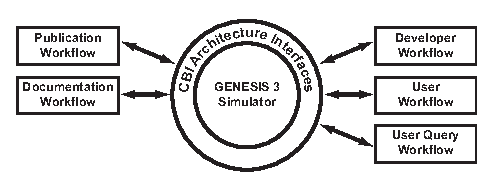
\includegraphics[scale=1.5]{figures/G3-global-workflows.eps}
%\caption{{\bf A Dummy Figure:} Example of \LaTeX\,\,\,code to incorporate a figure into documentation.}
  \label{fig:wf-1}
\end{figure}

\subsection*{Documented Workflows}
Currently, the following workflows have been identified and documented:
\begin{itemize}
\item \href{../workflow-user/workflow-user.tex}{\bf User}
\item \href{../workflow-user-query/workflow-user-query.tex}{\bf User Question}
\item \href{../workflow-developer/workflow-developer.tex}{\bf Developer}
\item \href{../workflow-documentation/workflow-documentation.tex}{\bf Documentation}
\end{itemize}
\end{document}
